\chapter{RF-Score-v4: pose generation error}

\section{Abstract}

In prospective virtual screening, accurate prediction of binding affinity of docked poses is crucial for ranking compounds. However, many existing studies focus on scoring crystal complexes only, without considering the impact of pose generation error. Therefore the high accuracy claimed in those studies would potentially lead to degradation of predictive performance when their methods are applied to scoring docked poses.

In this study we investigate the impact of pose generation error on the predictive performance of both classical and machine-learning scoring functions. We also study their capability of predicting the near-native pose that is most conformationally closest to the crystal pose. Our results show that pose generation error affects the accuracy of scoring functions, which is well anticipated. To minimize this negative impact, re-training the scoring functions on docked poses instead of crystal poses can be a straightforward solution. On the other hand, we find that although machine-learning scoring functions are generally good at binding affinity prediction, they do not perform as well as classical scoring functions on native pose prediction. This indicates that predictions of binding affinity and native pose are two different tasks and no single scoring function performs optimally for both tasks.

This was a collaborative project with Pedro J. Ballester from Cancer Research Center of Marseille, Marseille, France. It was published in the \textit{Proceedings of the 11th International Meeting on Computational Intelligence Methods for Bioinformatics and Biostatistics (CIBB)} on 26 June 2014 \citep{1434}.

\section{Introduction}

Protein-ligand docking predicts the binding conformation (pose) of a ligand when bound to a target protein to form a stable complex, as well as their binding affinity. The former process is known as pose generation and the latter is known as scoring. There have been quite some studies \citep{1432,1433} on scoring crystal complexes. These studies only concentrate on crystal complexes in order to avoid confounding factors introduced by pose generation, therefore their methods and conclusions are only applicable to scoring crystal complexes. However, scoring of the docked poses of a molecule is required when the experimentally determined pose is not available. This is the common case in prospective virtual screening, such as our istar web service. Hence accurate prediction of binding affinity of a docked pose can be practically meaningful in sorting candidate compounds in a database.

Here we study the impact of pose generation error on classical and machine-learning scoring functions. Furthermore, we investigate which of these scoring functions is the most suitable for predicting the near-native pose, i.e. the docked pose most similar to the crystal pose. This kind of capability is referred to as ``docking power" in some other studies \citep{1411}.

This study can be regarded as an extension to the previous chapter \citep{1433}. The same models, materials and metrics were reused, with some slight adjustments specificially for the purpose of this study. Likewise, the numerical experiments were performed with AutoDock Vina \citep{595} as the classical scoring function because it is one of the most popular docking software, and RF-Score \citep{564} as the machine-learning scoring function because it has been vigorously studied in multiple aspects \citep{1281,1362,1370}. It is out of the scope of this study to investigate the generalization of the results to other machine learning methods such as support vector regression, but we expect them to yield similar conclusions.

\section{Methods}

We reused the four models, the two benchmarks, and the four performance measures described in the previous chapter. Here we only highlight the differences that were made particularly for investigating the imapct of pose generation error. For this purpose, new experiments were designed to generate and measure docked poses.

\subsection{Model 1 - AutoDock Vina}

Vina's score for the $k$th pose of a molecule is given by the predicted free energy of binding to the target protein and computed in Vina as:

\begin{equation}
\label{rfscore4:e_k}
e_k=\frac{e_{k,inter}+e_{k,intra}-e_{1,intra}}{1+w_6N_{rot}}
\end{equation}

Unlike the previous chapter, where $k=1$ because only the crystal pose was considered, in this study we aim at docked poses and thus $k$ can be an arbitrary value. Therefore $e_{k,intra}$ and $e_{1,intra}$ cannot be cancelled out. As a result, five more features from $e_{k,intra}$ were incorporated in models 2, 3 and 4, constituting a feature vector of 11 elements.

\subsection{Model 2 - MLR::Vina}

This is a multiple linear regression (MLR) model using the 11 unweighted Vina terms as features. Similarly, in order to make the problem amenable to MLR, we made a grid search on the $w_6$ weight and thereafter ran MLR on the remaining ten weights. The sampling range for $w_6$ was extended to [0.000 to 0.030] with a step size of 0.001 because of more variability when multiple docked poses were considered.

\subsection{Model 3 - RF::Vina}

This is a random forest (RF) model with the 11 Vina features using the default 500 trees and mtry values from 1 to 11. The selected model was the one that provided the lowest RMSE on the OOB (Out of Bag) data. This process was repeated ten times with ten different random seeds because RF is stochastic.

\subsection{Model 4 - RF::VinaElem}

This is an extension to RF::Vina and incorporates the 36 RF-Score features. Hence, it was built with 47 features. This process was also repeated ten times with ten different random seeds.

\subsection{The PDBbind benchmark}

We reused the PDBbind v2007 benchmark because the four models have been evaluated on it in the previous chapter, permitting a direct comparison. Briefly, the test set comprises 195 diverse complexes with measured binding affinities spanning more than 12 orders of magnitude, whereas the training set comprises 1105 non-overlapping complexes.

\subsection{The 2013 blind benchmark}

We reused the PDBbind v2013 blind benchmark because the four models have been evaluated on it in the previous chapter, allowing a direct comparison. Briefly, the test set comprises 382 complexes newly added in the 2013 release, whereas the training set comprises 2897 complexes from PDBbind v2012 refined set.

\subsection{Performance measures}

We reused the four performance measures: root mean square error RMSE, standard deviation SD, Pearson correlation coefficient Rp and Spearman correlation coefficient Rs between predicted and measured binding affinity. Note that RMSE was not calculated in a linear correlation, while SD was.

\subsection{Experimental design}

To generate docked poses, each ligand in the two benchmarks was docked into the binding site of its target protein using Vina. This process is known as redocking. As usual \citep{1362}, the search space was defined first by finding the smallest cubic box that covers the entire ligand and then by extending the box in X, Y, Z dimensions by 10\AA. Redocking a ligand resulted in up to nine docked poses output by Vina.

Here we define two schemes to refer to different poses from which the features are extracted. In scheme 1, the chosen pose is the crystal pose. In scheme 2, the chosen pose is the docked pose with the best Vina score, i.e. the one with the lowest Vina score in terms of estimated free energy. We trained the four models on both crystal and docked poses (in both schemes), and tested them also on both crystal and docked poses (in both schemes). Hereafter whenever we mention the docked pose, we implicitly refer to the one with the best Vina score, if not specified explicitly.

\section{Results}

After redocking by Vina, we used root mean square deviation (RMSD) to quantify the pose generation error, i.e. how different the 3D geometry of the redocked pose is from the corresponding crystal pose of the same ligand molecule. A RMSD value of 2\AA\ was used as a publicly accepted positive control for correct bound structure prediction. 101 out of the 195 ligands (52\%) in the PDBbind v2007 benchmark and 219 out of the 382 ligands (57\%) in the PDBbind v2013 blind benchmark had their best-scoring docked pose with RMSD < 2\AA. When all the docked poses (up to nine) were considered, these redocking success rates increased to 76\% and 81\%, respectively. These results are consistent with those obtained in \citep{1362}, where Vina managed to predict a conformation sufficiently close to that of the co-crystallized ligand as the first conformation in over half of the cases.

Tables \ref{rfscore4:tbl-set-1-pdbbind-2007} and \ref{rfscore4:tbl-set-2-pdbbind-2012} enumerate the predictive performance of the four models trained on crystal and docked poses and tested also on crystal and docked poses on the PDBbind v2007 benchmark and the PDBbind v2013 blind benchmark, respectively. Figures \ref{rfscore4:set-1-pdbbind-2007} and \ref{rfscore4:set-2-pdbbind-2012} plot the same results graphically, where trn-1 means the model was trained in scheme 1, i.e. on crystal poses, and trn-2 means the model was trained in scheme 2, i.e. on docked poses. Likewise, tst-1 and tst-2 mean the model was tested on crystal and docked poses, respectively. Note that model 1 was trained on crystal poses and used out of the box without re-training, so its results of trn-1 are simply repeated for trn-2.

\begin{table}
\caption{Performance of the four models trained on crystal and docked poses and tested also on crystal and docked poses on the PDBbind v2007 benchmark.}
\label{rfscore4:tbl-set-1-pdbbind-2007}
\begin{tabular}{cccrrrr}
\hline
Model & Training & Test & RMSE & SD & Rp & Rs\\
\hline
1 & Crystal & Crystal & 2.41 & 1.99 & 0.554 & 0.608\\
2 & Crystal & Crystal & 1.88 & 1.85 & 0.630 & 0.680\\
3 & Crystal & Crystal & 1.66 & 1.59 & 0.744 & 0.752\\
4 & Crystal & Crystal & 1.52 & 1.42 & 0.803 & 0.799\\
\hline
1 & Crystal & Docked  & 2.02 & 1.98 & 0.557 & 0.597\\
2 & Crystal & Docked  & 1.90 & 1.87 & 0.622 & 0.670\\
3 & Crystal & Docked  & 1.76 & 1.72 & 0.693 & 0.710\\
4 & Crystal & Docked  & 1.60 & 1.52 & 0.772 & 0.771\\
\hline
2 & Docked  & Crystal & 1.91 & 1.88 & 0.618 & 0.648\\
3 & Docked  & Crystal & 1.74 & 1.69 & 0.705 & 0.716\\
4 & Docked  & Crystal & 1.58 & 1.45 & 0.794 & 0.790\\
\hline
2 & Docked  & Docked  & 1.86 & 1.83 & 0.640 & 0.667\\
3 & Docked  & Docked  & 1.69 & 1.63 & 0.730 & 0.730\\
4 & Docked  & Docked  & 1.55 & 1.45 & 0.795 & 0.789\\
\hline
\end{tabular}
\end{table}

\begin{table}
\caption{Performance of the four models trained on crystal and docked poses and tested also on crystal and docked poses on the PDBbind v2013 blind benchmark.}
\label{rfscore4:tbl-set-2-pdbbind-2012}
\begin{tabular}{cccrrrr}
\hline
Model & Training & Test & RMSE & SD & Rp & Rs\\
\hline
1 & Crystal & Crystal & 2.30 & 1.81 & 0.406 & 0.414\\
2 & Crystal & Crystal & 1.67 & 1.67 & 0.535 & 0.521\\
3 & Crystal & Crystal & 1.54 & 1.54 & 0.629 & 0.593\\
4 & Crystal & Crystal & 1.43 & 1.43 & 0.689 & 0.662\\
\hline
1 & Crystal & Docked  & 1.87 & 1.78 & 0.437 & 0.432\\
2 & Crystal & Docked  & 1.70 & 1.69 & 0.520 & 0.505\\
3 & Crystal & Docked  & 1.61 & 1.60 & 0.585 & 0.549\\
4 & Crystal & Docked  & 1.49 & 1.49 & 0.656 & 0.633\\
\hline
2 & Docked  & Crystal & 1.69 & 1.69 & 0.521 & 0.509\\
3 & Docked  & Crystal & 1.62 & 1.61 & 0.580 & 0.560\\
4 & Docked  & Crystal & 1.48 & 1.47 & 0.669 & 0.650\\
\hline
2 & Docked  & Docked  & 1.68 & 1.68 & 0.524 & 0.509\\
3 & Docked  & Docked  & 1.59 & 1.59 & 0.594 & 0.553\\
4 & Docked  & Docked  & 1.47 & 1.48 & 0.665 & 0.643\\
\hline
\end{tabular}
\end{table}

\begin{figure}
\centering
\subfloat{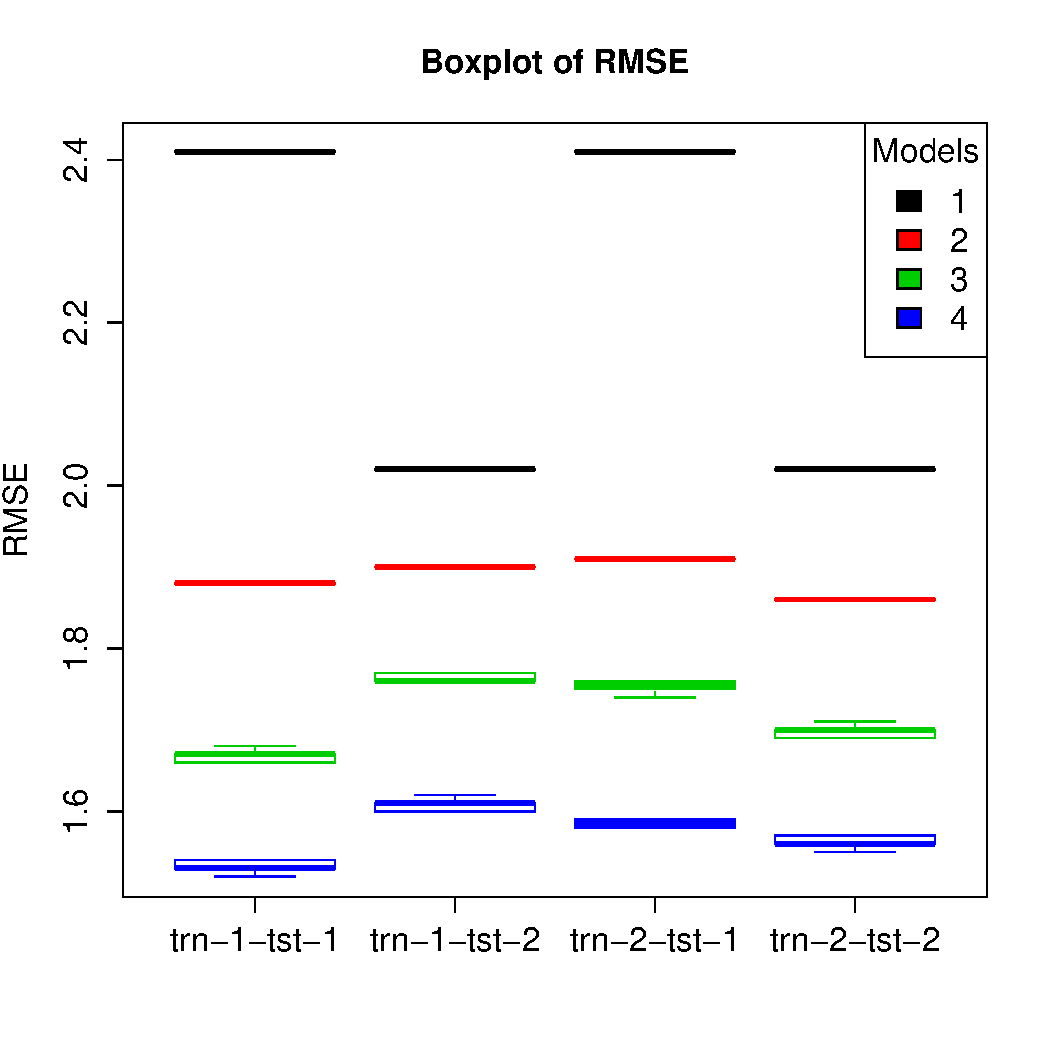
\includegraphics[width=0.48\linewidth]{../rfscore4/set-1-pdbbind-2007-rmse-boxplot.pdf}}
\subfloat{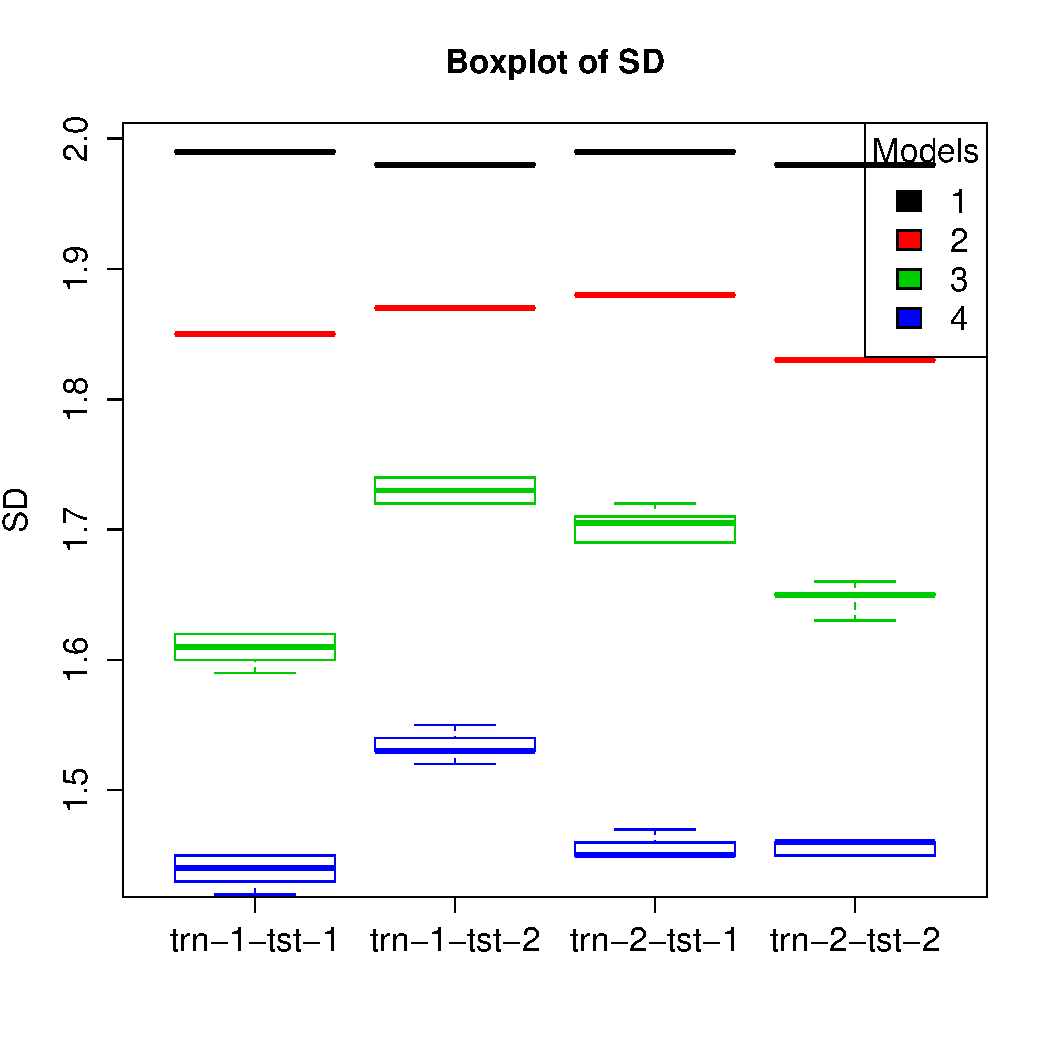
\includegraphics[width=0.48\linewidth]{../rfscore4/set-1-pdbbind-2007-sdev-boxplot.pdf}}
\\
\subfloat{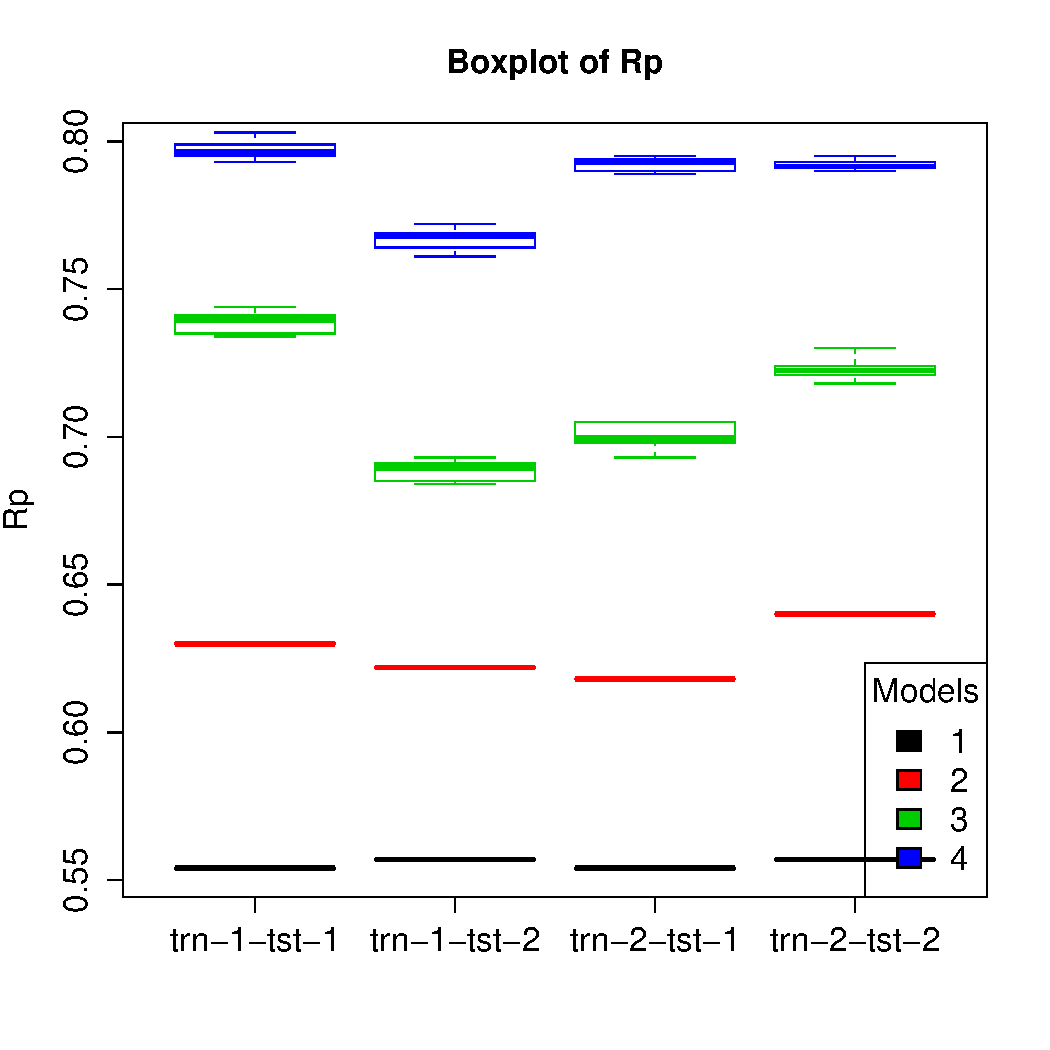
\includegraphics[width=0.48\linewidth]{../rfscore4/set-1-pdbbind-2007-pcor-boxplot.pdf}}
\subfloat{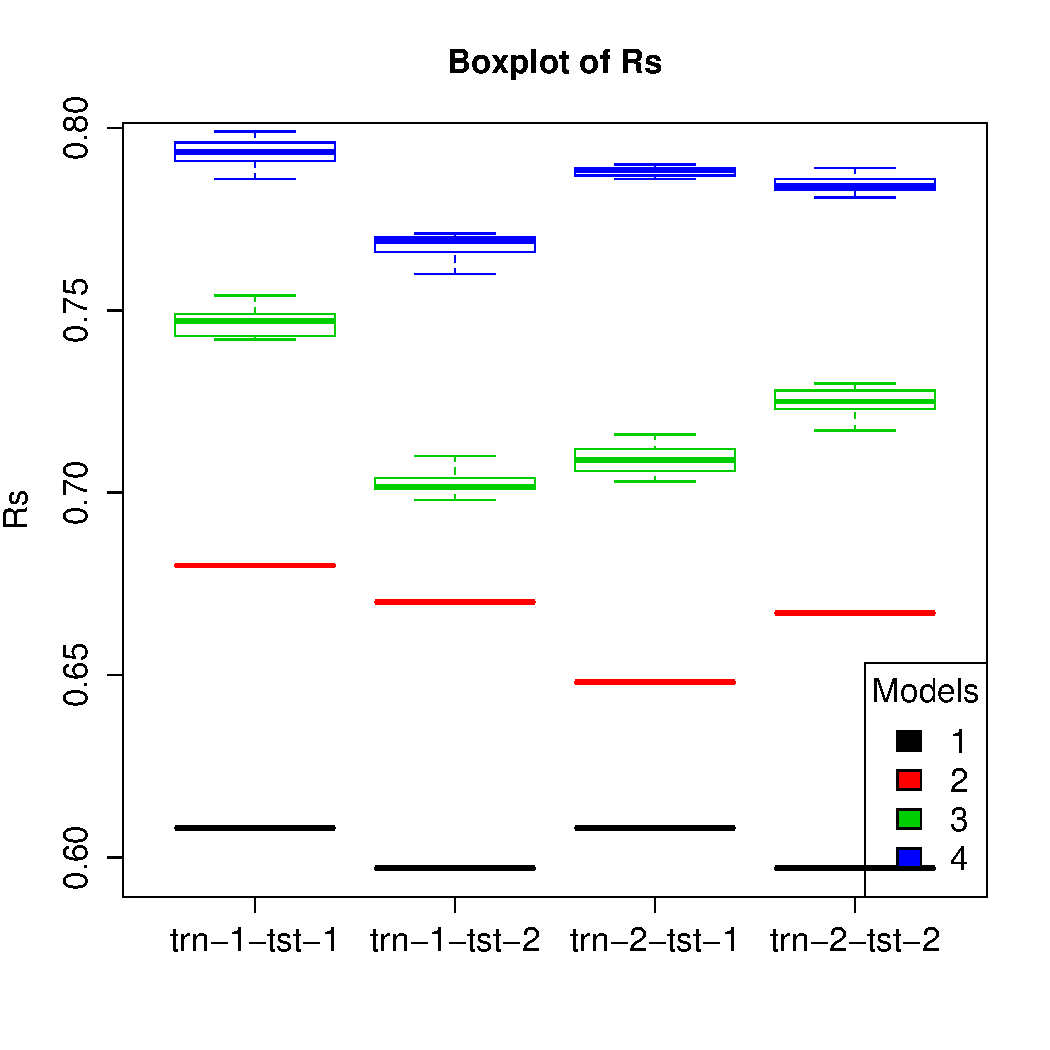
\includegraphics[width=0.48\linewidth]{../rfscore4/set-1-pdbbind-2007-scor-boxplot.pdf}}
\caption{Performance of the four models trained on crystal and docked poses and tested also on crystal and docked poses on the PDBbind v2007 benchmark.}
\label{rfscore4:set-1-pdbbind-2007}
\end{figure}

\begin{figure}
\centering
\subfloat{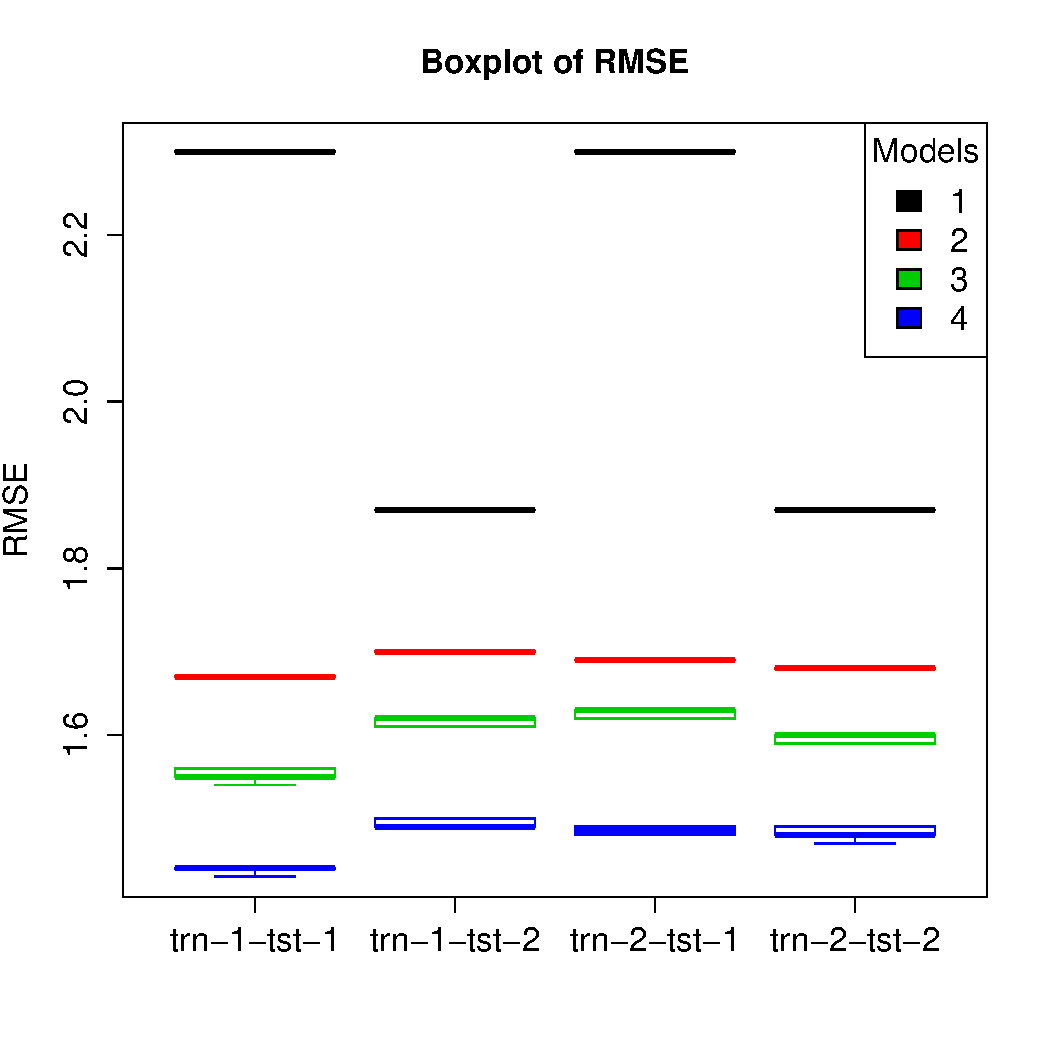
\includegraphics[width=0.48\linewidth]{../rfscore4/set-2-pdbbind-2012-rmse-boxplot.pdf}}
\subfloat{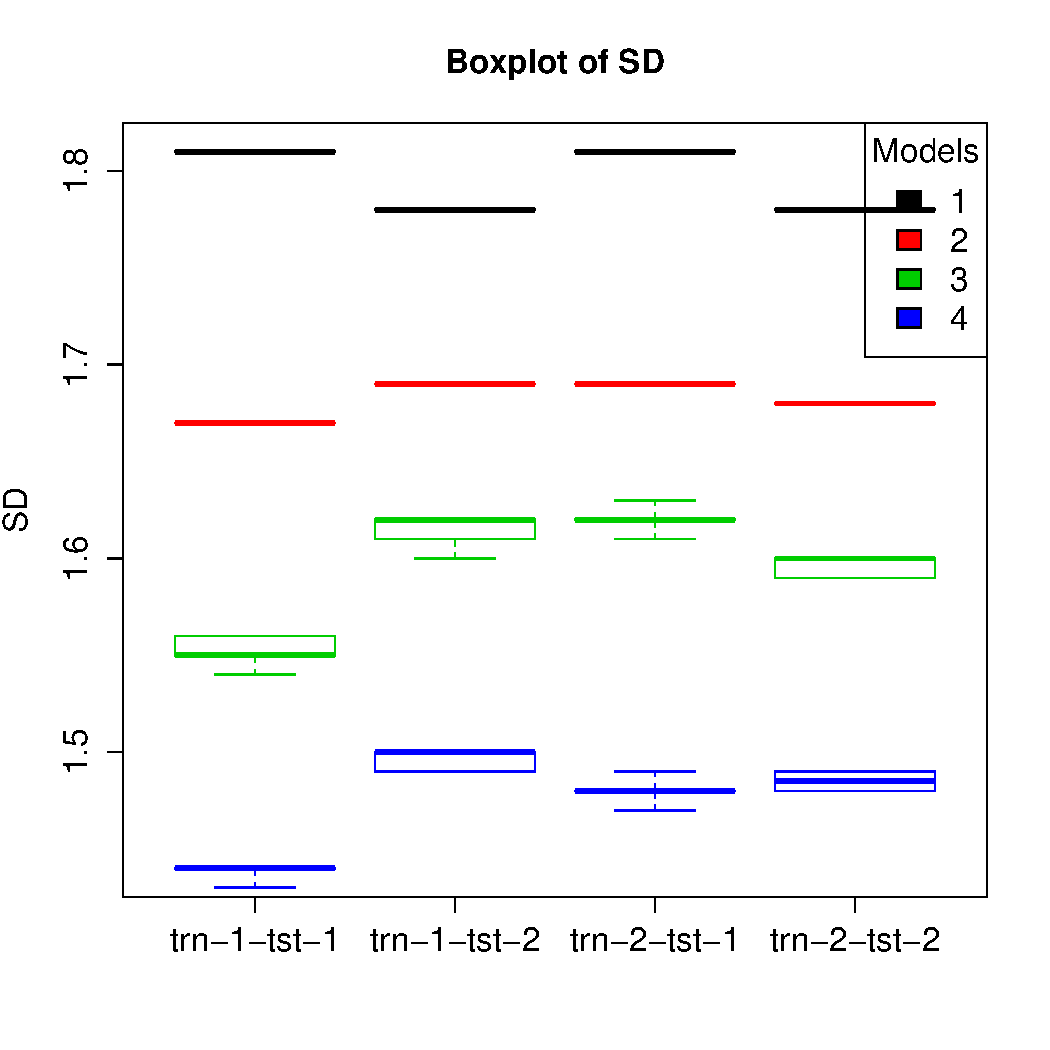
\includegraphics[width=0.48\linewidth]{../rfscore4/set-2-pdbbind-2012-sdev-boxplot.pdf}}
\\
\subfloat{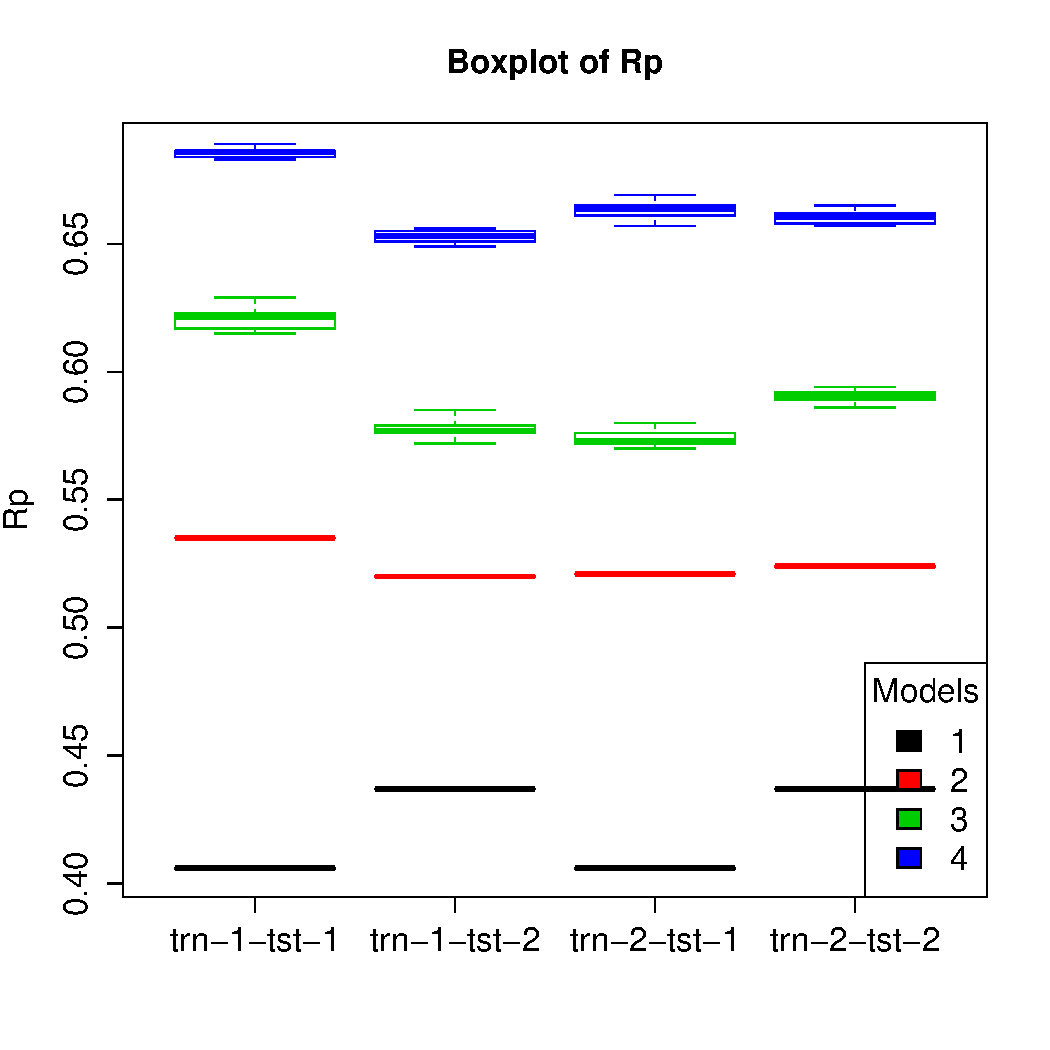
\includegraphics[width=0.48\linewidth]{../rfscore4/set-2-pdbbind-2012-pcor-boxplot.pdf}}
\subfloat{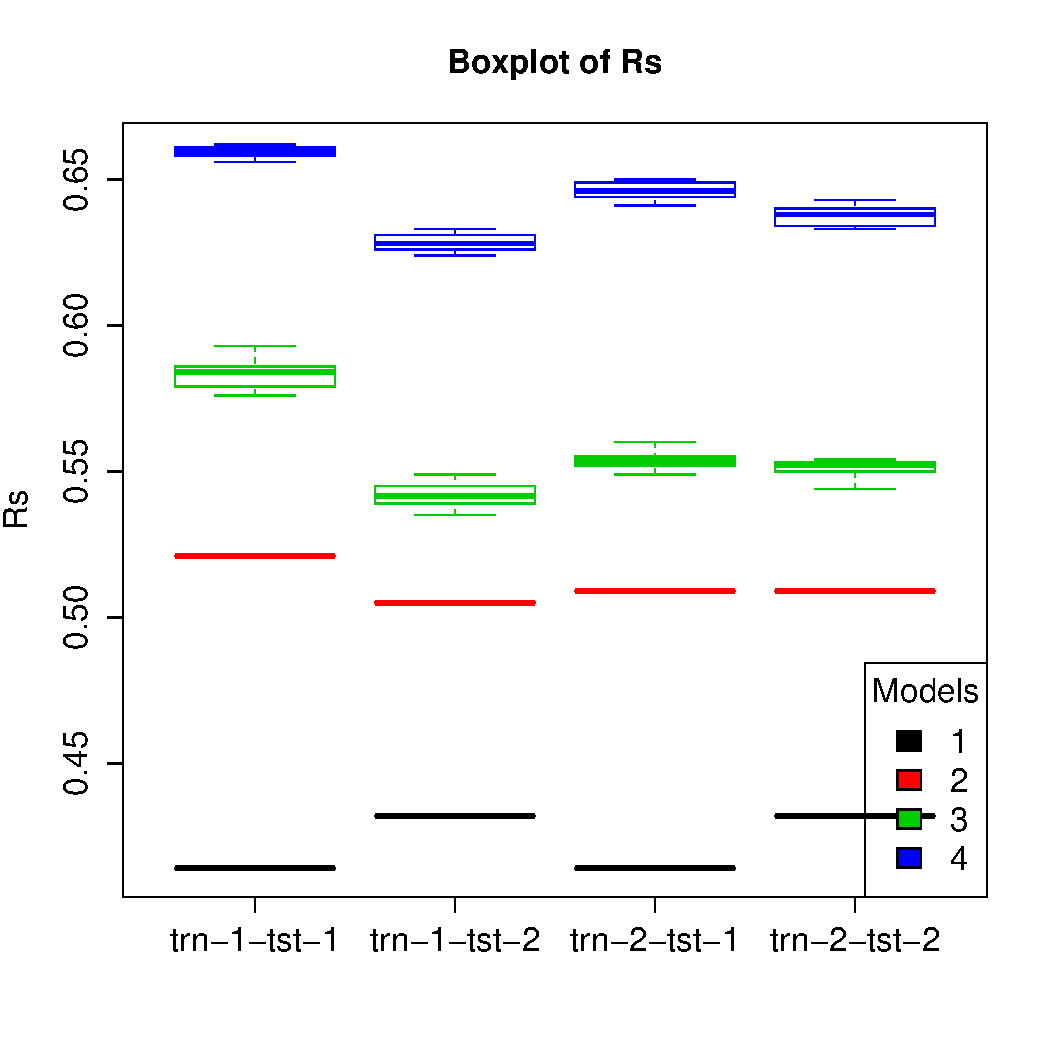
\includegraphics[width=0.48\linewidth]{../rfscore4/set-2-pdbbind-2012-scor-boxplot.pdf}}
\caption{Performance of the four models trained on crystal and docked poses and tested also on crystal and docked poses on the PDBbind v2013 blind benchmark.}
\label{rfscore4:set-2-pdbbind-2012}
\end{figure}

From these results on both benchmarks, several interesting phenomena are observed. First, for model 1, its performance tested on docked poses was always better than its performance tested on crystal poses, except for the Rs performance on the PDBbind v2007 benchmark. Vina performing better on docked poses is likely to be due to the fact that docked poses are by construction optima of the objective function spanned by the Vina score, which may favor prediction of docked poses over unoptimized crystal poses.

Second, for models 2, 3 and 4 trained on crystal poses, their performance tested on docked poses was always worse than their performance tested on crystal poses. This is well anticipated because of the impact of pose generation error.

Third, for models 2, 3 and 4 tested on docked poses, their performance was better when they were trained on docked poses than their counterparts trained on crystal poses. This implies that a simple and quick solution to improving performance on docked poses is to re-train the model on docked poses instead of on crystal poses.

Fourth, for models 2, 3 and 4 tested on crystal poses, the models trained on docked poses did not outperform their counterparts trained on crystal poses. This is also well anticipated due to the impact of pose generation error, and suggests that it is not feasible to improve the predictive performance on crystal poses by using docked poses for training.

Fifth, regardless of the training or test schemes, model 4 consistently outperformed model 3, which in turn outperformed model 2, which in turn outperformed model 1. It is remarkable that the best scoring function, RF::VinaElem, when trained on docked poses, achieved the highest performance in the literature on the PDBbind v2007 benchmark in the more common application of re-scoring docked poses. Here we denote this version of RF::VinaElem as RF-Score-v4 specifically for the purpose of binding affinity prediction given a docked pose. Importantly, since Vina and RF::Vina used the same features and were trained on the same data, RF::Vina performed much better in predicting binding affinity than the widely-used Vina while having the same applicability domain.

Next, we assessed the ability of each of the four models to predict the near-native pose from the up to nine docked poses output by Vina (Table \ref{rfscore4:near-native}). In other words, we would like to see if a model could correctly assign the best score to the particular docked pose having the lowest RMSD to the crystal pose out of at most nine docked poses. Interestingly, results show that Vina, although being the least accurate predictor of binding strength, turned out to be the best at predicting which docked pose is geometrically the closest to the crystal pose. This is probably due to the fact that, as explained previously, the best-scoring docked pose was resulted from optimization of Vina's scoring function during redocking. In contrast, the presented machine-learning scoring functions, while excelling at binding affinity prediction, performed much worse than Vina at native pose prediction. This indicates that these two tasks, binding affinity prediction and native pose prediction, cannot be optimally covered by a single scoring function.

\begin{table}
\caption{Near-native pose prediction.}
\label{rfscore4:near-native}
\begin{tabular}{ccccc}
\hline
& \multicolumn{2}{c}{PDBbind v2007 benchmark} & \multicolumn{2}{c}{PDBbind v2013 blind benchmark}\\
Model & \# & \% & \# & \%\\
\hline
1 & 94 & 48 & 208 & 54\\
2 & 59 & 30 & 142 & 37\\
3 & 53 & 27 & 119 & 31\\
4 & 59 & 30 & 141 & 37\\
\hline
\end{tabular}
\end{table}

\section{Conclusions}

This study has demonstrated that errors in pose generation generally introduce a degradation in the accuracy of scoring. One straightforward approach to enhancing predictive accuracy on docked poses is to re-train the scoring function also on docked poses. Furthermore, RF-Score-v4, essentially RF::VinaElem trained on docked poses, obtained the highest predictive performance on two PDBbind benchmarks in the common scenario where one has to predict the binding affinity of docked poses instead of those for crystal poses, usually because a crystal structure of the ligand is unavailable. Nevertheless, we observed that the presented machine-learning scoring functions did not perform as well as Vina in predicting the near native pose of a ligand. This could be due to the confounding factor that the docked poses were all generated and optimized by Vina.

\section{Future works}

The redocking experiment was carried out by Vina in this study. It is of great interest to repeat the experiment with idock to see if the same conclusions still hold. If so, we can substitute RF-Score-v4 for RF-Score-v3 in our istar web platform for large-scale prospective virtual screening.

\chapterend
